%%%%%%%%%%%%%%%%%%%% author.tex %%%%%%%%%%%%%%%%%%%%%%%%%%%%%%%%%%%
%
% sample root file for your "contribution" to a contributed volume
%
% Use this file as a template for your own input.
%
%%%%%%%%%%%%%%%% Springer %%%%%%%%%%%%%%%%%%%%%%%%%%%%%%%%%%


% RECOMMENDED %%%%%%%%%%%%%%%%%%%%%%%%%%%%%%%%%%%%%%%%%%%%%%%%%%%
\documentclass[graybox]{svmult}

% choose options for [] as required from the list
% in the Reference Guide

\usepackage{mathptmx}       % selects Times Roman as basic font
\usepackage{helvet}         % selects Helvetica as sans-serif font
\usepackage{courier}        % selects Courier as typewriter font
\usepackage{type1cm}        % activate if the above 3 fonts are
                            % not available on your system
%
\usepackage{makeidx}         % allows index generation
\usepackage{graphicx}        % standard LaTeX graphics tool
                             % when including figure files
\usepackage{multicol}        % used for the two-column index
\usepackage[bottom]{footmisc}% places footnotes at page bottom

% see the list of further useful packages
% in the Reference Guide

\usepackage{listings}
\usepackage{color}
\definecolor{lightgray}{rgb}{.9,.9,.9}
\definecolor{darkgray}{rgb}{.4,.4,.4}
\definecolor{purple}{rgb}{0.65, 0.12, 0.82}

\lstdefinelanguage{JavaScript}{
  keywords={typeof, new, true, false, catch, function, return, null, catch, switch, var, if, in, while, do, else, case, break},
  keywordstyle=\color{blue}\bfseries,
  ndkeywords={class, export, boolean, throw, implements, import, this},
  ndkeywordstyle=\color{darkgray}\bfseries,
  identifierstyle=\color{black},
  sensitive=false,
  comment=[l]{//},
  morecomment=[s]{/*}{*/},
  commentstyle=\color{purple}\ttfamily,
  stringstyle=\color{red}\ttfamily,
  morestring=[b]',
  morestring=[b]"
}

\lstset{
   language=JavaScript,
   backgroundcolor=\color{lightgray},
   extendedchars=true,
   basicstyle=\footnotesize\ttfamily,
   showstringspaces=false,
   showspaces=false,
   numbers=none,
   numberstyle=\footnotesize,
   numbersep=9pt,
   tabsize=2,
   breaklines=true,
   showtabs=false,
   captionpos=b
}



\makeindex             % used for the subject index
                       % please use the style svind.ist with
                       % your makeindex program

%%%%%%%%%%%%%%%%%%%%%%%%%%%%%%%%%%%%%%%%%%%%%%%%%%%%%%%%%%%%%%%%%%%%%%%%%%%%%%%%%%%%%%%%%

\begin{document}

\title*{Media Synchronization on the Web}
% Use \titlerunning{Short Title} for an abbreviated version of
% your contribution title if the original one is too long
\author{Ingar M. Arntzen, Nj{\aa}l T. Borch and Fran\c{c}ois Daoust}
% Use \authorrunning{Short Title} for an abbreviated version of
% your contribution title if the original one is too long
\institute{Ingar M. Arntzen \at Norut Northern Research Institute, Troms{\o}, Norway \email{ingar.arntzen@norut.no}
\and Nj{\aa}l T. Borch \at Norut Northern Research Institute, Troms{\o}, Norway \email{njaal.borch@norut.no}
\and Fran\c{c}ois Daoust \at World Wide Web Consortium (W3C), Paris, France \email{fd@w3.org}}

\maketitle

% abstract
\abstract{
The Web is a natural platform for multimedia, with universal reach, powerful
backend services and a rich selection of components for capture, interactivity
and presentation. In addition, with a strong commitment to modularity,
composition and interoperability, the Web should allow advanced media
experiences to be constructed by harnessing the combined power of simpler
components. Unfortunately, with timed media this may be complicated, as media
components require synchronization to provide a consistent experience. This is
particularly the case for distributed media experiences.

In this chapter we focus on temporal interoperability on the Web, how to allow
heterogeneous media components to operate consistently together, synchronized
to a common timeline and subject to shared media control. A programming model
based on external timing is presented, enabling modularity, interoperability
and precise timing among media components, in single-device as well as multi-device 
media experiences. The model has been proposed within the W3C Multi-device 
Timing Community Group as a new standard, and this could establish
temporal interoperability as one of the foundations of the Web platform.

}

\begin{keywords}
media synchronization, media orchestration, motion model, timing object, multi-device
\end{keywords}

% introduction
\section{Introduction}
\label{sec:intro}
The Web is all about modularity, composition and interoperability, and this
applies across the board, from HTML-based layout and styling to JavaScript-
based  tools and frameworks. Unfortunately, there is a notable exception to
this rule. Composing presentations from multiple, timed media components is
far from easy. For instance, consider a Web page covering motor sport, using
Web Audio~\cite{webaudio} for sound effects and visuals made from HTML5
videos, a map with timed GPS-data, WebGL~\cite{webgl} for timed infographics,
a timed Twitter~\cite{twitter} widget for social integration, and finally an
iframed ad-banner for paid advertisements timed to the race.

In this chapter we focus on media synchronization challenges of this kind,
making multiple, heterogeneous media components operate consistently with
reference to a common timeline, as well as common media control. This, we call
\emph{temporal interoperability}. Lack of support for temporal
interoperability represents a significant deviation from the core principles
of the Web. Harnessing the combined powers of timed media components
constitutes a tremendous potential for Web-based media experiences, both in
single-device and multi-device scenarios.

The key to temporal interoperability is finding the right approach to media
synchronization. There are two basic approaches; \emph{internal
timing} or \emph{external timing}. Internal timing
is the familiar approach, where media components are coordinated by
manipulating their control primitives. External timing is the
opposite approach, where media components are explicitly designed to be parts
of a bigger experience, by accepting direction from an external timing source.

Though internal timing is currently the predominant approach in Web-
based media, external timing is the key to temporal interoperability;
If multiple media components are connected to the same external timing source,
synchronized behavior across media components follows by implication. This
simplifies media synchronization for application developers. Furthermore,
by allowing external timing sources to be synchronized and shared across a
network, external timing is also a gateway to precise distributed multimedia
playback and orchestration on the Web platform.

This chapter provides an introduction to external timing as well as the
flexible media model and programming model that follows from this approach,
proposed for standardization within the \emph{W3C Multi-device Timing
Community Group (MTCG)}~\cite{mtcg} to encourage temporal interoperability on
the Web platform. The \emph{timing object} is the central concept in this
initiative, defining a common interface to external timing and control for the
Web. The MTCG has published a draft specification for the timing
object~\cite{timingobject} and also maintains
\emph{Timingsrc}~\cite{timingsrc}, an open source JavaScript implementation of
the timing object programming model. The chapter also describes the
\emph{motion model}, which provides online synchronization of timing objects.

The chapter is structured as follows: Sect.~\ref{sec:mediasync} defines media
synchronization as a term and briefly presents common challenges for
synchronization on the Web. The motion model is presented in
Sect.~\ref{sec:model}. 
Sect.~\ref{sec:interoperability} TODO.
Sect.~\ref{sec:web} surveys the abilities and limitations of Web technologies with respect to media synchronization.
Sect.~\ref{sec:motion} gives an introduction to the motion concept, and to programming with motions, including synchronization of AV media and timed data.
Sect.~\ref{sec:motionsync} distributed
synchronization of motions
Evaluation is presented in Sect.~\ref{sec:eval}.
Sect.~\ref{sec:standard} briefly references the standardization initiative
made by the Multi-device Timing Community Group~\cite{mtcg}, before
conclusions are given in Sect.~\ref{sec:concl}.


% terminology
\section{Central Terms}
\label{sec:terms}
This section lists central terms used in this chapter.

\runinhead{Timeline:} 

logical axis for media presentation. Values on the timeline are usually
associated with a unit, e.g. seconds, milliseconds, frame count or slide
number. Timelines may be infinite, or bounded by a range (i.e minimum and
maximum values).

\runinhead {Clock:} 

a point moving predictably along a timeline, at a fixed, positive rate.
Hardware clocks ultimately depend on a crystal oscillator. System clocks
typically count seconds or milliseconds from \emph{epoch} (i.e. 1. Jan 1970
UTC), and may be corrected by clock synchronization protocols (e.g.
NTP~\cite{ntp}, PTP~\cite{ptp}). From the perspective of application
developers, the value of a clock may be read, but not altered.

\runinhead {Motion:} 

a unifying concept for \emph{media playback} and \emph{media control}. Motion
represents a point moving predictably along a timeline, with added support for
flexibility in movement and interactive control. Motions support discrete
jumps on the timeline, as well as a variety of continuous movements expressed
through velocity and acceleration. Not moving (i.e. paused) is considered a
special case of movement. Motion is a generalization over classical concepts
in multimedia, such as \emph{clocks}, \emph{media clocks}, \emph{timers},
\emph{playback controls}, \emph{progress}, etc. Motions are implemented by an
\emph{internal clock} and a \emph{vector} describing current movement (position,
velocity, acceleration), timestamped relative to the internal clock.
Application developers may update the movement vector of a motion at any time.

\runinhead {Timed data:} 

data whose temporal validity is defined in reference to a timeline. For
instance, the temporal validity of subtitles are typically expressed in terms
of points or intervals on a media \emph{timeline}. Similarly, the temporal validity
of video frames essentially maps to frame-length intervals. Timed scripts are
a special case of timed data where data represents functions, operations or
commands to be executed.


\runinhead {Continuous media:} 

Typically audio or video data. More formally, a subset of \emph{timed data}
where media objects cover the timeline without gaps.


\runinhead {Media component:} 

essentially a player for some kind of timed data. Media components are based
on two basic types of resources: timed data and motion. The timeline of timed
data must be mapped to the timeline of motion. This way, motion defines the
temporal validity of timed data. At all times, the media component works to
produce correct media output in the UI, given the current state of timed data
and motion. A media component may be anything from a simple text animation in
the \emph{Document Object Model (DOM)}, to a highly sophisticated media framework.


\runinhead {User agent:} 

any software that retrieves, renders and facilitates end user interaction with
Web content, or whose user interface is implemented using Web technologies.

\runinhead {Browsing context:} 

JavaScript runtime associated with Web document. Browser windows, tabs or
\emph{iframes} each have their own browsing context.

\runinhead {Iframe:} 

Web document nested within a Web document, with its own browsing context.


% media synchronization
\section{Media Synchronization}
\label{sec:mediasync}
Dictionary definitions of \emph{media synchronization} typically refer to
presentation of multiple instances of media at the same time. A related term
is \emph{media orchestration}, possibly emphasizing more the importance of
media control and planned scheduling of media playback. Similarly, we have
used the term \emph{media timing} to highlight the universal utility of clocks
in digital media, for capture, control, synchronization, timeshifting,
scheduling and playback. In this chapter we use the term \emph{media
synchronization} in a broad sense, as a synonym to \emph{media orchestration}
and \emph{media timing}. We also limit the definition in two regards:

\begin{itemize}
\item{Media synchronization on the Web is clock-based. The latencies and heterogeneity of the Web environment requires a clock-based approach for acceptable synchronization quality.}
\item{Media synchronization involves one media instance and a clock. The term relative synchronization is reserved for comparisons between media instances.}
\end{itemize}

\subsection{Challenges}


\begin{table}
\centering
\caption{Common challenges for media synchronization on the Web.}
\label{tab:challenges}
\setlength{\tabcolsep}{10pt}
\begin{tabular}{cc}
\hline\noalign{\smallskip}
Synchronization challenges & Use-cases \\
\noalign{\smallskip}\svhline\noalign{\smallskip}
across media sources & multi-angle video, ad-insertion \\
across media types & video, WebAudio, animated map \\
across iframes & video, timed ad-banner \\
across tabs, browsers, devices & split content, interaction \\
across platforms & Web, native, broadcast \\
across people and groups & collaboration, social \\
across Internet & global media experiences \\
\noalign{\smallskip}\hline\noalign{\smallskip}
\end{tabular}
\end{table} 



Media synchronization has a wide range of use-cases on the Web, as illustrated
by Table~\ref{tab:challenges}. Well known use-cases for synchronization within
a single Web page include multi-angle video, accessibility features for video,
ad-insertion, as well as media experiences spanning different media types,
media frameworks, or iframe boundaries. Synchronization across Web pages allow
Web pages to present alternative views into a single experience; dividing or
duplicating media experiences across devices. Popular use-cases in the home
environment involve collaborative viewing, multi-speaker audio, or big screen
video synchronized with related content on handheld devices. Use-cases towards
the end of the list target global scenarios, such as distributed capture and
synchronized Web visualizations for a global audience.

\subsection{Approach}

The challenges posed by all these use-cases may be very different in terms of
complexity, requirements for precision, scale, infrastructure and more. Yet,
we argue that a single solution is needed. Implementing specific solutions for
specific use-cases is very expensive and time-consuming, and lays heavy
restrictions on reusability. Even worse, circumstances regarding
synchronization may change dynamically during a media session. For instance, a
smartphone involved in synchronization over the local network, will have to
switch approach for synchronization once the user leaves the house, or
switches from WiFi to the mobile network. Crucially though, by solving media
synchronization across Internet, all challenges listed above are solved by
implication. For instance, if video synchronization is possible across Web
pages on the Internet, then synchronizing two videos within the same Web page
is just a special case. It follows that the general solution to media
synchronization on the Web is distributed and global in nature. Locality may
be exploited for synchronization, yet only as optimization.


% motion model
\section{The Motion Model}
\label{sec:model}
The primary objectives of the motion model are global synchronization,
\emph{Web availability} and simplicity for Web developers. Global
synchronization implies media synchronization across the Internet. Web
availability means that no additional assumptions can be introduced for media
synchronization. If a Web browser is able to load an online Web page, it
should also be able to synchronize correctly. The model proposed for this can
be outlined in three simple steps:

\begin{itemize}
\item{Media clock and media controls are encapsulated in one concept, and
represented as a stateful resource. This chapter uses the term \emph{motion}\footnote{\emph{motion} as in \emph{motion pictures}. \emph{Moving through media} still remains a good way to conceptualize media experiences, not least as media experiences become virtual and immersive.
} for this
concept.} 
\item{A \emph{motion} is an online resource, implying that it is hosted by a
server and identifiable by URLs.}
\item{\emph{Media components}\footnote{\emph{media component:} anything from a simple $<div>$ tag with text, to a highly sophisticated media player or multimedia framework.
} synchronize themselves relative to online motions.}
\end{itemize}

According to the model, media synchronization should be a consequence of
connecting multiple media components to the same online motion. This way, rich
synchronized multi-device presentation may be crafted by connecting relevant
media components to the same online motion. 

\begin{figure}[h]
%\sidecaption
\centering
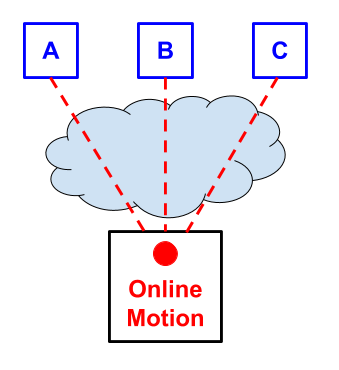
\includegraphics[scale=.4]{fig/motion-model.png}
\caption{Media components on three different devices (A,B,C), all connected to an online motion
(red circle). Media control requests (e.g. pause/resume) target the online motion and are transmitted across the Internet (light blue cloud). The corresponding state change is
communicated back to all connected media components. Each media component
adjusts its behaviour independently.}
\label{fig:model}
\end{figure}

Importantly, the practicality of the motion model depends on Web developers
being shielded from the complexities of distributed synchronization. This is
achieved by having a \emph{timing object} locally in the Web browser. The
timing object acts as an intermediary between media components and online
motions, as illustrated by Fig.~\ref{fig:model-2}. This way, the challenge of
media synchronization is divided in two parts.

\begin{itemize}
\item{\emph{motion synchronization}: timing object precisely synchronized with online motion (Internet problem).}
\item{\emph{component synchronization}: media component precisely synchronized with timing objects (local problem).} 
\end{itemize}


\begin{figure}[h]
%\sidecaption
\centering
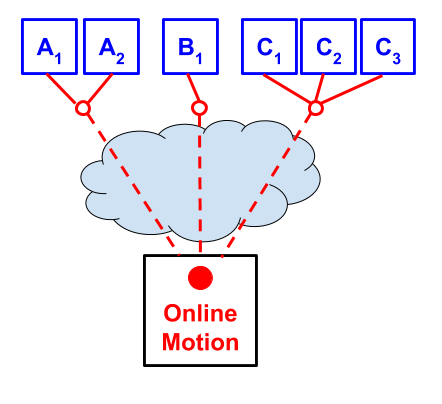
\includegraphics[scale=.4]{fig/motion-model-2.png}
\caption{Timing objects (red unfilled circles) mediate access to online motion. Timing objects may be shared by independent mediacomponents within the same browser context.}
\label{fig:model-2}
\end{figure}

\emph{Motion synchronization} ensures that timing objects connected to the
same online motion are kept precisely synchronized. The logic required for
motion synchronization could be supported by Web browsers natively (if
standardized), or imported into Web pages as an third party JavaScript
library. Motion synchronization is outlined in Sect.~\ref{sec:motionsync}.

\emph{Component synchronization} implies that a media component continuously strives
to synchronize its activity relative to a timing object. As such, component
synchronization is a local problem. Media components always interface with
timing objects through a well defined \emph{API} (see Sect.~\ref{sec:motionapi}).
Sect.~\ref{sec:compsync} discusses component synchronization in
further detail.


% temporal interoperability
\section{Temporal Interoperability}
\label{sec:interoperability}
Temporal interoperability implies that multiple, possibly heterogeneous media
components may easily be combined into a single, consistently timed media
experience. We argue that temporal interoperability must be promoted as a
principal feature of the Web, and finding the right approach to media
synchronization is key to achieving this. In this section we distinguish two
basic approaches, \emph{internal timing} and \emph{external timing}, and
explain why external timing is better suited as a basis for temporal
interoperability. Notice that timing is provided by motions according to the
motion model.

\begin{figure}[h]
%\sidecaption
\centering
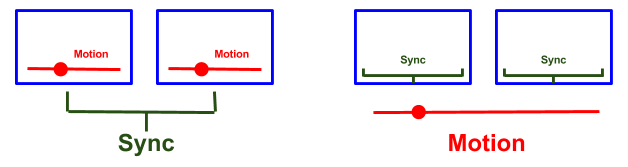
\includegraphics[scale=.4]{fig/internal-external.png}
\caption{
	Blue rectangles represent media components, red symbols represent motion, and green symbols represent the process of media synchronization. To the left; internal timing and external media synchronization. To the right; external timing and internal media synchronization.
}
\label{fig:internalexternal}
\end{figure}


\subsection{Internal timing}

Internal timing is the most familiar one, where media components are typically
media players or frameworks internalizing aspects of timing and control.
Synchronizing such media components is an external process, utilizing the
control primitives provided by each component.

Internal timing means that media components implement timed operations
internally, based on the system clock or some other (hardware) timer and state
representing motion. Timed operations may also be affected by other internal
factors, such as the buffering of timed data, time consumption in processing,
or delays in UI pipelines. The outside world is typically given access to the
internal motion of the media component via interactive elements in the UI, or
programmatically through control primitives defined in the component API. For
example, the HTML5 media element allows media playback to be requested by
clicking the play button or invoking the play method. The media element then
organizes media playback in its own time, subject to delays in initialisation
procedures, buffering, decoding and AV-subsystems.

\subsection {External timing}

External timing is the opposite approach, where media components consider
themselves parts of a bigger experience. Such media components are explicitly
designed to take direction from an external motion, and always do their best
to synchronize their own behavior accordingly. If multiple media components
are connected to the same external motion, synchronized behavior across media
components follows by implication. In this approach, media synchronization is
redefined as an internal challenge, to be addressed by each media component
independently.


\runinhead{Media control:}

The external timing approach implies that control over the media component is
exercised indirectly, by manipulating the external motion instead of the media
component. For instance, if the external motion is paused or time-shifted, the
media component must react accordingly. Appropriate controls for the media
component may still be exposed through the UI or API of the component.
However, such control requests must be routed to the external motion. This
ensures that control applies to all media components connected to the same
external motion. It also ensures that media components may process control
requests without regard to the origin of the request. Importantly, media
components directed by external motions may still make use of an internal
clock. Importantly though, the external motion takes precedence, so deviations
must be compensated for by adjusting the internal clock.

\runinhead{Precision:}

Precision is a key ambition in media synchronization. With internal timing,
synchronization with other media is performed using the control primitives
that each media component defines. In the Web environment, such control
primitives have typically not been designed with precise timing in mind  (see
Sect.~\ref{sec:web-html}).  This makes high quality synchronization hard to
achieve. In this model media synchronization generally gets more difficult as
the number of components increases. Heterogeneity in media types and control
interfaces complicate matters further. For precise synchronization, external
timing appears to be a better approach. Media synchronization is solved
internally in media components, where it can be implemented with unrestricted
access to the internal state and capabilities of the component. Furthermore,
the synchronization task is shifted from external application developers to
the author of the media component. This makes sense, as the author likely has
better understanding of how the media component works. It also ensures that
the problem may be solved once, instead of repeatedly by different application
developers.


\runinhead{Buffering:}

Another distinctive feature of the external motion approach is that motion is
not sensitive to the internal state (e.g. data availability) of any media
component. For instance, external motion might describe playback while a
particular media component still lacks data. In the external motion approach,
media components must always align themselves with the external motion, to the
best of their abilities. For example, media components may adapt by buffering
data further ahead, changing to a different data source (e.g. lower bitrate)
or even changing to a different presentation mode (e.g audio only). This way,
playback may continue undisturbed and media components join in as soon as they
are able to. This is particularly important in multi-device scenarios, where a
single device with limited bandwidth might otherwise hold back the entire
presentation. On the other hand, if the readiness of a particular media
component is indeed essential to the experience, this may be solved in
application code, by pausing and resuming the external motion.


\runinhead{Master-Slave:}

Asymmetric master slave synchronization is a common pattern in media
synchronization. The pattern implies that internal motion of a master media
component is used as external motion for slave media components. However, with
multiple media components all but one must be a slave. In the external timing
approach all media components are slaves, and the external motion itself is
the master. This avoids added complexities of the master-slave  pattern, and
provides a symmetric model where each media component may request control via
the external motion. On the other hand, if asymmetry is indeed appropriate for
a given application, this may easily be emulated. For instance, applications
may ensure that only one specific media component may issue control requests
to the external motion.

\runinhead{Live and on-demand:}

Solutions for live media often target minimized transport latency for real-time 
presentation. In other words, the internal motion of live media
components is tied to data arrival. This may be problematic in some
applications, as differences in transport latency imply that media components
will be out of sync. For example, live Web-based streaming solutions may be
seconds apart, even on the same network. Timing issues with live media is even
more evident in rich media productions involving multiple live feeds with very
different production chains and transport mechanisms. The external timing
approach provides the control and flexibility needed for applications to deal
with these realities in appropriate ways. With an external motion representing
the official live motion, multiple live media sources may be presented in a
time-consistent way across components and screens. Such a live motion could be
selected to cover at least a majority of viewers. Furthermore, inability to
follow the official live motion would be detected by media components
internally, potentially triggering application specific reactions. For
instance, the viewer could be prompted to switch to a private, slightly time-shifted 
motion suitable for his or her specific environment.



% state of the Web
\section{State of the Web}
\label{sec:web}
\newpage

% motion
\section{Motion}
\label{sec:motion}
Motion is a simple concept representing playback state (media clock), as well
as functions for accessing and manipulating this state (media controls). As
such, similar constructs are found in most multimedia frameworks.

\begin{figure}[h]
%\sidecaption
\centering
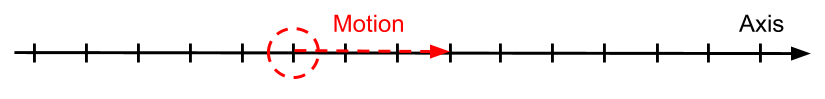
\includegraphics[scale=.4]{fig/motion-axis.png}
\caption{Motion: point moving along an axis. The current position
is marked with a red circle (dashed), and forward velocity of 3 units per second is
indicated by the red arrow (dashed).}
\label{fig:motion}
\end{figure}

As illustrated in Fig.~\ref{fig:motion}, motion represents movement (in real-time)
of a point, along an axis (timeline). At any moment the point has well
defined position, velocity and acceleration\footnote{Some animation frameworks
support acceleration. Acceleration broadens the utility of motions, yet will
likely be ignored in common use cases in classical media (see
Section~\ref{sec:toomuch}).}. Velocity and acceleration describe continuous
movements. Velocity is defined as position-change per second, whereas
acceleration is defined as position- change per second squared. Discrete jumps
on the timeline are also supported, simply by modifying the position of the
motion. A discrete jump from position A to C implies that the transition took
no time, and that no position B (between A and C) was visited. Not moving
(i.e. zero velocity and acceleration) is a special case of movement.

\runinhead{Internal State.}
\label{sec:internalstate}
Motion is defined by an internal clock and a vector (position, velocity,
acceleration, timestamp). The vector describes the initial state of the
current movement, timestamped relative to the internal clock. This way, future
states of the motion may be calculated precisely from the initial vector and
elapsed time. Furthermore, application programmers may control the motion
simply by supplying a new initial vector. The motion concept was first
published under the name Media State Vector (MSV)~\cite{msv}.


\subsection{Timing object API}
\label{sec:motionapi}

Timing objects provide access to motions. Timing objects may be constructed
with a URL to an online motion. If the URL is omitted, it will represent a
local motion instead.

\begin{lstlisting}[caption=Constructing a timing object.]
var URL = "...";
var timingObject = new TimingObject(URL);
\end{lstlisting}

The \emph{Timing object API} defines two operations, \emph{query} and
\emph{update}, and emits a \emph{change} event as well as a periodic
\emph{timeupdate} event.


\runinhead{query():} 

The query operation returns a vector representing the current state of the
motion. This vector includes position, velocity and acceleration, as well as a
timestamp. For instance, if a query returns position 4.0 and velocity 1.0 and no acceleration, a
new query one second later will return position 5.0.

\begin{lstlisting}[caption=Querying the timing object to get a snapshot vector.]
var v = timingObject.query();
console.log("pos:" + v.position);
console.log("vel:" + v.velocity);
console.log("acc:" + v.acceleration);
\end{lstlisting}


\runinhead{update(vector):} 

The update operation accepts a vector parameter specifying new values for
position, velocity and acceleration. This initiates a new movement for the
motion. Omitting say position implies that the current position will be used.
So, an update with velocity 0 pauses the motion at the current position.

\begin{lstlisting}[caption=Updating the timing object.]
// play, resume
timingObject.update({ velocity: 1.0 }); 
// pause
timingObject.update({ velocity: 0.0 });
// jump and play from 10
timingObject.update({ position: 10.0, velocity: 1.0});
// jump to position 10, keeping the current velocity
timingObject.update({ position: 10.0 });
\end{lstlisting}


\runinhead{timeupdate event:}

For compatibility with existing HTML5 media elements and an easy way to update graphical elements, a \emph{timeupdate} evens is emitted periodically.

\runinhead{change event:}

Whenever a motion is updated, event listeners on the timing object (i.e. media components)
will immediately be invoked. Note that the \emph{change} event is not emitted
periodically like the \emph{timeupdate} event of HTML5 media elements. The change event signifies the start of a
new movement, not the continuation of a movement.



\begin{lstlisting}[caption=Monitoring changes to the motion through the change event.]
timingObject.on("change", function (e) {
  var v = motion.query();
  if (v.velocity === 0.0 && v.acceleration === 0.0) {
    console.log("I'm not moving!");
  } else {
    console.log("I'm moving!");
  }
});
\end{lstlisting}




\subsection{Programming with motions}


\runinhead{Using motions:}

Motions are resources used by Web applications, and the developer may define
as many as required. What purposes they serve in the application is up to the
programmer. If the motion should represent media offset in milliseconds, just
set the velocity to 1000 (advances the position of the motion by 1000
milliseconds per second). Or, for certain musical applications it may be
practical to let the motion represent beats per second.

\runinhead{Timing converters:}

A common challenge in media synchronization is that different sources of media
content may reference different timelines. For instance, one media stream may
have a logical timeline starting with 0, whereas another is timestamped with
epoch values. If the relation between these timelines is known (i.e.
\emph{relative skew}), it may be practical to create a skewed timing object
for one of the media components, connected to the motion. This is supported by
\emph{timing converters}. Multiple timing converters may be connected to a
motion, each implementing different transformations such as scaling and
looping. Timing converters may also be chained. Timing converters implement
the \emph{timing object API}, so media components can not distinguish between
a timing object and a timing converter. A number of timing converters are
implemented in the Timingsrc programming model~\cite{timingsrc}.

\runinhead{Flexibility:}
\label{sec:toomuch}

The mathematical nature of the motion concept makes it flexible, yet for a
particular media component some of this flexibility may be unnecessary, or
even unwanted. For instance, the HTML5 media player will typically not be able
to operate well with negative velocities, very high velocities, or with
acceleration. Fortunately, it does not have to. Instead, the media player may
define alternative modes of operation as long as the motion is in an
unsupported state. It could show a still image every second for high velocity,
or simply stop operation altogether (e.g. black screen with error message).
Later, when motion re-enters a supported state, normal operation may be
resumed for the media player.


\subsection{Online Motion}
\label{sec:motionsync}

The timing object API is particularly designed to mediate access to online motions,
as illustrated by Fig.~\ref{fig:model-repeat}. \emph{Update} operations are forwarded to the
online motion, and will not take effect until notification is received from
the online motion and \emph{change events} are emitted. In contrast, \emph{query} is a local
(and cheap) operation. This ensures that media components may sample the
motion frequently if needed. So, through the Timing Object API, online motions
are made available to Web developers as local objects. Only the latency of the
update operation should be evidence of a distributed nature.

\begin{figure}[h]
%\sidecaption
\centering
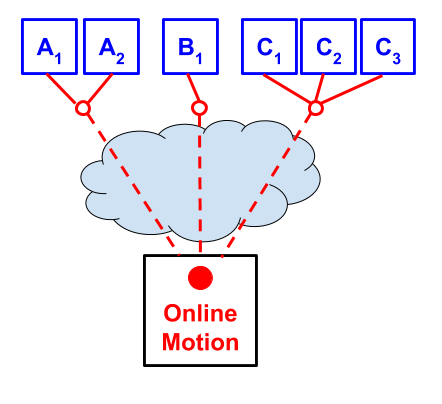
\includegraphics[scale=.3]{fig/motion-model-2.png}
\caption{(Fig.~\ref{fig:model-2} repeated for convenience.) Timing objects (red unfilled circles) mediate access to online motion. Timing objects may be shared by independent media components within the same browsing context.}
\label{fig:model-repeat}
\end{figure}

To support this abstraction, precise, distributed \emph{motion
synchronization} is required. In particular, the internal \emph{clock} of the
motion must be precisely synchronized with the clock at the online motion
server. Synchronized system clocks (e.g. \emph{Network Time Protocol (NTP)}~\cite{ntp} or \emph{Precision Time Protocol (PTP)}~\cite{ptp}) is
generally not a valid assumption in the Web domain.  As a consequence, an
alternative method of estimating a shared clock needs to be used, for example
by sampling an online clock directly. In addition, low latency is important
for user experiences. Web agents should be able to join synchronization
quickly on page load or after page reload. To achieve this, joining agents
must quickly obtain the current vector and the synchronized clock. For some
applications the user experience might also benefit from motion updates being
disseminated quickly to all agents. Web agents should also be able to join and
leave synchronization at any time, or fail, without affecting the
synchronization of other agents. Motion synchronization is discussed in more
detail in~\cite{msv}.

\emph{InMotion} is a hosting service for online motions, built by the Motion Corporation~\cite{mcorp}. A dedicated onlice service supporting
online motions is likely key to achieving non-functional goals, such as
high availability, reliability and scalability. Evaluation of
motion synchronization is presented in Section~\ref{sec:eval}.

Finally, the timing object API emphasizes an attractive programming model for
multi-device media applications. In particular, by making online motions
available under the same API as local motions (see Section~\ref{sec:motionapi}),
media components may be used in single-page as well as multi-device media
experiences, without modification. Also, by hiding the complexity of
distributed motion synchronization, application developers may focus on
building great media components using the timing object API. As such, the
timing object API provides much needed separation of concern in multi-device
media.

\subsection{Synchronizing Audio and Video}
\label{sec:avsync}

On the Web, playback of audio and video is supported by HTML5 media
elements~\cite{html5media}. Synchronizing media elements relative to a timing
object means that the \emph{currentTime} property (i.e. media offset) must be
kept equal to the position of the timing object at all times, at least to a
good approximation. The general approach is simply to monitor the media
element continuously, and try to rectify whenever the synchronization error
grows beyond a certain threshold. For larger errors \emph{seekTo} is used. This is
typically the case on \emph{page load}, or after timing object \emph{change} events. Smaller
errors are rectified gradually by manipulating \emph{playbackrate}. \emph{SeekTo} is
quite disruptive to the user experience, so support for variable \emph{playbackrate}
is currently required for high quality synchronization.

\emph{MediaSync} is a JavaScript library allowing HTML5 media elements to be
synchronized by timing objects. The MediaSync library targets usage across the
most common Web browsers, so it is not optimized for any particular scenario.
Though synchronization of HTML5 media is simple in theory, it involves a few
practical challenges, as indicated in Section~\ref{sec:web-html}. First,
\emph{currentTime} is only a coarse representation of the media offset, and it
fluctuates considerably when compared to the system clock. The MediaSync
library solves this by collecting a backlog of samples, from which a value of
currentTime can be estimated. Building up this backlog requires some samples,
so it may take more than a second for estimates to stabilize. Another issue
relates to unpredictable time-consumption in media control operations. In
particular, seekTo(X) will change currentTime to X, but it will require a non-negligible 
amount of time to do so. In the context of synchronization, it aims
for a fixed target when it should be aiming for a moving target. The MediaSync
library compensates for this by overshooting the target. Furthermore, in order
to overshoot by the correct amount, the algorithm collects statistics from
every seekTo operation. Surprisingly perhaps, this strategy works reasonably
well. Evaluation for the MediaSync library is presented in Section~\ref{sec:eval}.


\subsection{Synchronizing timed data}
\label{sec:sequencer}

Synchronization of timed data using timing objects is an important challenge.
Timed data such as subtitles, tracks, scripts, logs or time series typically
include items tied to \emph{points} or \emph{intervals} on the timeline.
Synchronization then involves activating and deactivating such items at the
correct time, in reference to a timing object. To simplify programming of
media components based on timed data, a generic \emph{Sequencer} is defined.
The sequencer is similar to the HTML5 track element~\cite{html5track}, but is
directed by the timing object instead of a HTML5 media
element~\cite{html5media}. Web developers register cues associated with
intervals on the timeline, and receive event upcalls whenever a cue is
activated or deactivated. The sequencer fully supports the timing object,
including skipping, reverse playback and acceleration. It may be used for any
data type and supports dynamic changes to cues during playback.

\begin{figure}[h]
%\sidecaption
\centering
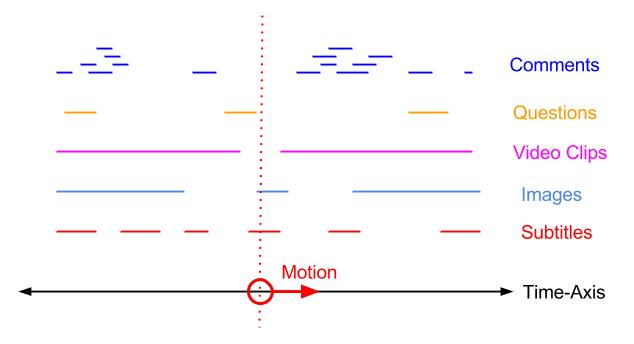
\includegraphics[scale=.4]{fig/sequencer.jpg}
\caption{Five data sources of timed data, with items tied to intervals on the timeline. Motion along the same timeline defines which items are active (vertical dotted line), and precisely when items will be activated or deactivated.}
\label{fig:sequencer}
\end{figure}


The sequencer is implemented as a JavaScript library and made available as
part of the open-source \emph{Timingsrc}~\cite{timingsrc} programming model
(see Section~\ref{sec:standard}). In the interest of precisely synchronized
activation and deactivation and low CPU consumption, the sequencer
implementation is not based on frequent polling. Instead, the deterministic
nature of the timing object allows events to be calculated and scheduled using
\emph{setTimeout}, the timeout mechanism available in Web browsers. Though
this mechanism is not optimized for precision, Web browsers may be precise
down to a few milliseconds. The sequencer is presented in further detail in~\cite{sequencer}.








% flexibility
\section{Flexibility and Extensibility}
\label{sec:flexibility}
Modern multimedia increasingly demands high flexibility and extensibility.
This is driven by a number of strong trends: device proliferation, new
sensors, new data types (e.g. sensor data, 3D, 360 video), multiple data
sources, live data, personalization, interactivity, responsiveness and multi-device 
support. On top of all this there are also rising expectations to UI
design, integration with social networks, and more.

In an attempt to meet such demands, new features have been added to media
frameworks allowing programmers to customize the media player to a larger
extent. For example, the Flash~\cite{flash} framework has grown increasingly
feature-rich over time, even having partially overlapping features with the
Web platform itself. Media Source Extensions (MSE)~\cite{mse} in HTML5
provides a way to manipulate the video stream client-side. It is also common
for media players to expose events and timed cues, allowing custom
functionality to be implemented in application code. The text track system of
HTML5 is an example of this. MPEG-4~\cite{mpeg4} adds support for
synchronization and composition of multiple media streams, including timed data
such as graphical objects (2D and 3D). In particular, the MPEG-4 Systems
part~\cite{mpeg4sys} defines an architecture for media clients (terminals)
integrating a variety of media formats, delivery methods, interactivity and
rendering.

In short, the need for extensibility has driven a development towards
standardization of new data formats and features, leading media players to
become increasingly sophisticated, yet also more complicated and heavyweight.
We call this the \emph{big player} approach to flexibility and extensibility in
multimedia.


\subsection{Multiple small players}

The motion model presents an attractive alternative to the big player
approach. The key idea is that a big player may be replaced by multiple
smaller players, with precisely synchronized playback. As illustrated in
Fig.~\ref{fig:motion-media}, the flexibility of the motion model allows a
variety of specialized media components to be coupled together, forming custom
and complex media experiences from simpler parts.


\begin{figure}[h]
%\sidecaption
\centering
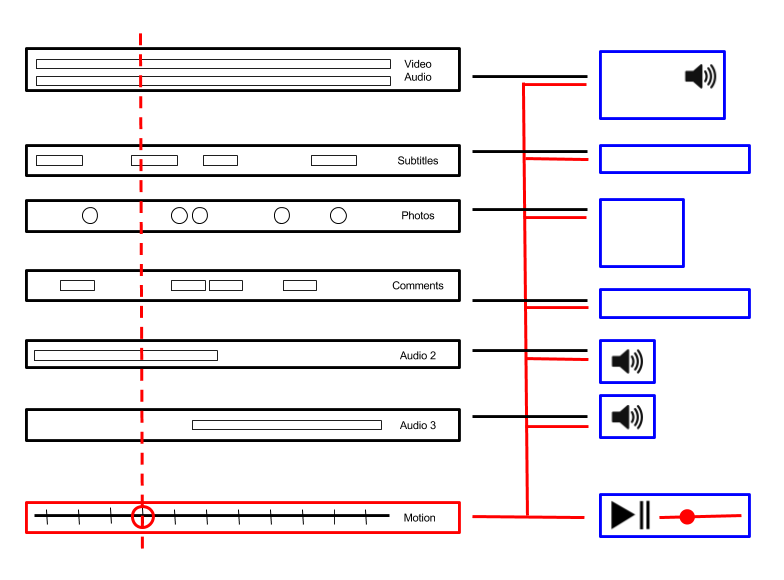
\includegraphics[scale=.4]{fig/motion-media.png}
\caption{A single media experience made from multiple media components (blue), possibly distributed across multiple devices. Each media component is connected to motion (red) and a source of timed data (black). There are different types of timed data: an AV container, a subtitle track, photos, comments and two extra audio tracks. The motion defines the timeline for the presentation, and timed data is mapped to this timeline by each media component. Since all the media components are connected to the same motion, they will operate in precise synchrony. One particular media component (bottom media element) provides interactive controls for the presentation, and connects only with motion.}
\label{fig:motion-media}
\end{figure}


\subsection{Dedicated media components}

The motion model typically encourage a pattern where each media
component is dedicated to solving a small and well defined challenge: Given
timed data, a motion and a DOM element, generate the correct presentation at
all times. Such custom media components are implemented in application code,
and an appropriate delivery method may be selected for the particular media
type and the task at hand. This way, application specific data formats may be
integrated into a presentation, as well as standardized formats. Importantly,
timed data sources may be dynamic and live, implying that presentations may
interact directly with live backend systems and update their presentations
during playback.

Media components may also be dedicated with respect to UI. For instance, a
single media component may implement interactive controls for the motion,
thereby relieving other media components from this added complexity. This
encourages a pattern where media components are designed for specific roles in
an application, e.g. controllers, viewers and editors, and combined to form
the full functionality. Of course, the fact that these media components are
independent may be hidden for end users with appropriate layout and styling,
giving the impression of a tightly integrated product. In any case, dedicated
media components may be reusable across different views, applications, devices
or data sets, as long as APIs to data model and motions remain unchanged.

\subsection{Flexible coupling}

The motion model allows modularity and flexibility by loose coupling of media
components. In fact, media components may be coupled only indirectly through
shared motions and shared data sources. This ensures that media components can
be added or removed dynamically during playback, or even fail, without
disrupting the rest of the presentation. This flexibility is also valuable in
development, as media components may be coded and tested in isolation or with
other components. New components may always be added without introducing any
additional increase in complexity, naturally supporting an incremental
development process. Also, the model does not impose restrictions on how
motions and timed data sources are connected with media components. A single
data source may be shared between multiple media components, or conversely, a
single media component may use multiple data sources. The same flexibility
goes for motions. There might be multiple aspects of timing and control in an
application, requiring multiple motions to be shared between media components.


\subsection{Client-side Synthesis}

Client-side synthesis is core design principle of the Web platform, and
central to key properties such as flexibility, extensibility, reusability and
scalability. This principle may now be fully exploited in the context of timed
media applications. With the motion model, timed media experiences
may be synthesised in real time within the browsing context (client-side), by
independent media components working directly on live data sources and
motions.

Interestingly, client-side synthesis is not the established approach to linear
media, not even in the Web context. With media frameworks such as Flash or
MPEG, media is typically assembled in a media file or media container, before
being uploaded or streamed to a client-side media player. Essentially, this is
server-side synthesis (and client-side playback). While server-side synthesis
may have certain advantages (e.g. robustness and simplicity), the
disadvantages are evident. By assembling data within media files and container
formats, data is decoupled from its source and effectively flattened into an
immutable copy. New media types must therefore often be addressed through
standardization of new media and container formats, and support must be
implemented by media players. This may be time-consuming process. That
said, server-side synthesis may still be an appropriate choice for a wide
range of media products.

Importantly though, in the motion model the choice between client-side 
synthesis and server-side synthesis is left to application programmers.
Established container-based media frameworks are still usable, provided only
that the framework can be integrated and controlled by external motion.
Ideally, this integration should be performed internally by the framework. If
this is done, frameworks can easily be used in conjunction with native media
elements, other frameworks or components that support external motion. If not,
integration may also be done externally, subject to the limitations of the
framework API. In any case, the motion model relieves media
frameworks from the challenge of doing everything, and highlights their value
as dedicated, reusable components.


% evaluation
\section{Evaluation}
\label{sec:eval}
The evaluation is concerned with feasibility of the motion model and
simplicity for Web developers.


\subsection {Motion Synchronization}

We have used motion synchronization for a wide range of technical
demonstration since 2010. An early evaluation of the research prototype is
discussed in the paper titled \emph{The Media State Vector}~\cite{msv}. Though
the interpretations of the experiments are conservative, early findings
indicated that motion synchronization could provide frame rate levels of
accuracy (33 milliseconds). A few years later, a production ready service
called \emph{InMotion} was built by spin off company Motion
Corporation~\cite{mcorp}. With the introduction of
WebSockets~\cite{websocket}, results improved significantly. Synchronization
errors are in the order of a few milliseconds on all major browsers and most
operating systems (including Android). Typically we observe 0-1 millisecond
errors for desktop browsers, compared to a system clock synchronized by NTP.
The \emph{InMotion} service has also been running continuously for years,
supporting a wide range of technical demonstrations, at any time, at any
place, and across a wide range of devices. As such, the value of a production
grade online service is also confirmed.

Furthermore, the precision of motion synchronization degrades well with poor
network conditions. For instance, experiments with video synchronization in \emph{Enhanced Data rates for GSM Evolution (EDGE)}
connectivity has not been visibly worse, except for longer update
latency. In this instance, video data was fetched from local files.
Conferences are also notorious hotspots for bad connectivity. In these
circumstances, availability of media data consistently fails before
synchronization.


\subsection {Synchronization of HTML5 media elements}

Two technical reports~\cite{syncreport1,syncreport2} document the abilities
and limitations of HTML5 media elements with respect to media synchronization,
as well the quality of synchronization achieved by the \emph{MediaSync}
library. Synchronization errors of about 7 milliseconds is reported for both
audio and video, on desktops, laptops and high-end smartphones. This
corresponds to echoless audio playback. Smartphones and embedded devices such
a ChromeCast can be expected to provide frame accurate synchronization. 

These results have been consistently confirmed by day to day usage over
several years. The user experience of multi-device video synchronization is
also very good, to the point that errors are hardly visible, as demonstrated by
this video~\cite{carneval}. Echoless synchronization with the MediaSync
library may also produce various audio effects, like failing to hear one audio
source, until volume levels are changed and only the other audio source can be
heard. Since these effects are also achieved across browser types and
architectures, this is a strong indication that external timing is feasible
and already at a useful level.

Synchronization has also been maintained for hours and days at end, without
accumulated errors. Loading speeds are also acceptable. Even though the
MediaSync library requires about 3 seconds to reach echoless, the experience
is perceived as acceptable much before this. A variety of video demonstrations
have been published at the Multi-device Timing Community Group
Website~\cite{mtcg}.

\begin{figure}[h]
%\sidecaption
\centering
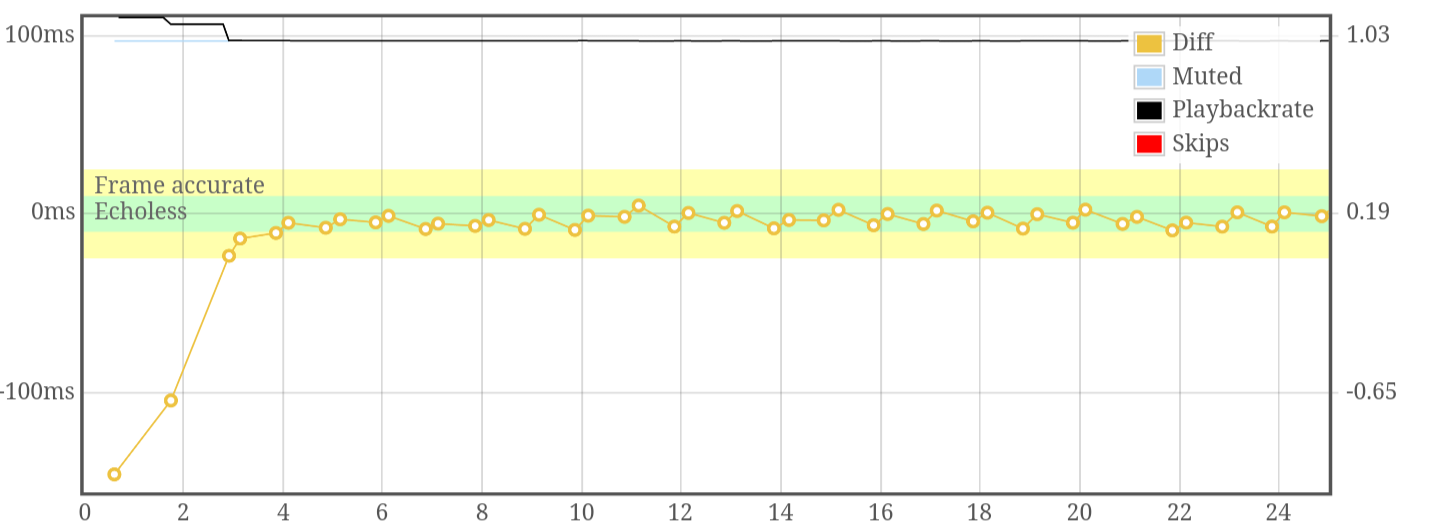
\includegraphics[scale=.23]{fig/android-video.png}
\caption{The figure illustrates an experiment with video (mp4) synchronization on
Android using Chrome browser. The plot shows currentTime compared to the ideal
playback position defined by motion. The X-axis denotes the timeline of the experiment (seconds).
The left Y-axis denotes difference \emph{Diff} (milliseconds) between currentTime and motion.
The green band (echoless) is +-10 millisecond and the yellow (frame accurate is) +-25 millisecond. 
This is achived using variable playbackRate. No skips were performed in this experiment. 
The right Y-axis denotes the value of playbackrate (seconds per second). The media element was muted until playbackrate stabilized.}
\label{fig:videosync}
\end{figure}

Though echoless synchronization is generally achievable, a lack of
standardization and common tests makes it impossible to provide any
guarantees. The experience might also be improved or become broken across
software updates. To be able to support echoless synchronization reliably
across browsers and devices, standards must include requirements for
synchronization, and testing-suites must be developed to ensure that those
requirements are met. Ideally though, media synchronization should be
implemented natively in media elements.


\subsection {Summary}

Interestingly, the results for motion synchronization and HTML5 media
synchronization are well aligned with current limitations of the Web platform.
For instance, the precision of timed operation in JavaScript is about 1
millisecond, and a 60Hz screen refresh rate corresponds to 16 milliseconds.
Furthermore, these results also match limitations in human sensitivity to
synchronization errors. 

Finally, programming synchronized media experiences in the motion model is
both easy and rewarding. In our experience, motions and sequencers are
effective thinking tools as well as programming tools. A globally synchronized
video experience essentially requires three code statements.

With this, we argue that the feasibility of the motion model is confirmed. It
is also clear that synchronization errors in online synchronization are
currently dominated by errors in synchronization in HTML5 media elements.
Future standardization efforts and optimizations would likely yield
significant improvements.

% standardization
\section{Standardization}
\label{sec:standard}
The Web is widely regarded as a universal multi-media platform. Yet, it still
lacks a common model for timing and media control. The motion model promises
to fill this gap, and indicates a significant potential for the Web as a
platform for globally synchronized capture and playback of timed multimedia.
To bring these possibilities to the attention of the Web community, the motion
model has been proposed for Web standardization. The Multi-device Timing
Community Group (MTCG)~\cite{mtcg} has been created to attract support for
this initiative. The MTCG has published the draft specification for the 
TimingObject~\cite{timingobject}. It has also published Timingsrc~\cite{timingsrc}, an open
source JavaScript implementation of the TimingObject specification, including
timing objects, timing converters, sequencers and the mediaSync library.

Though the ideas promoted by the MTCG have been received with enthusiasm by
members within the W3C and within the wider Web community, at present the MTCG
proposal has not been evaluated by the W3C.


% conclusions
\section{Conclusions}
\label{sec:concl}
We have explored media synchronization between heterogeneous media components,
and highlighted the need for temporal interoperability on the Web platform.
While internal timing is the popular approach to Web-based media, external
timing is the key to temporal interoperability.

This chapter provided an introduction to external timing as well as the media
model and the programming model that follows from this approach. By focusing
on modularity, loose coupling and client-side synthesis, this media model is
well aligned with key design principles of the Web, thereby fully extending
the flexibility and extensibility of the Web platform to timed Web
applications. Equally important, the external timing approach promises
precise distributed playback and media orchestration, enabling precise timing
and control also in multi-device Web-based media experiences.

To encourage temporal interoperability on the Web platform, the W3C Multi-
device Timing Community Group (MTCG)~\cite{mtcg} advocates standardization of
the timing object~\cite{timingobject} as a common interface to external timing
and control. Using the external timing approach, we have demonstrated that the
Web is already a strong platform for timed, multi-device media, though it was
not designed for it. With standardization it will become even better, likely
unleashing a new wave of Web-based creativity across a variety of application
domains.

Finally, as the external timing approach to media synchronization works on the
Web, it may also be ported to other native applications in the IP environment.
This provides a simple mechanism for making distributed media from a mixture
of native and Web-based media components.


% references
\newpage
\bibliographystyle{spmpsci}
\bibliography{chapter_v3} 

\end{document}
